%! Suppress = MissingImport
%%
%% sample document for AAMAS'19 conference
%%
%% modified from sample-sigconf.tex
%%
%% see ACM instructions acmguide.pdf
%%
%% AAMAS-specific questions? F.A.Oliehoek@tudelft.nl
%%

\pdfminorversion=7  %% Fixes .eps image files

\documentclass[sigconf]{aamas}  % do not change this line!
%% your usepackages here, for example:
\usepackage{booktabs}
\usepackage{listings}
\usepackage{graphicx}

%% do not change the following lines
\setcopyright{ifaamas}  % do not change this line!
\acmDOI{doi}  % do noadat change this line!
\acmISBN{}  % do not change this line!
\acmConference[AAMAS'20]{Proc.\@ of the 19th International Conference on Autonomous Agents and Multiagent Systems (AAMAS 2020), B.~An, N.~Yorke-Smith, A.~El~Fallah~Seghrouchni, G.~Sukthankar (eds.)}{May 2020}{Auckland, New Zealand}  % do not change this line!
\acmYear{2020}  % do not change this line!
\copyrightyear{2020}  % do not change this line!
\acmPrice{}  % do not change this line!


%% the rest of your preamble here
\lstset{
  basicstyle=\ttfamily,
  columns=fullflexible,
  frame=single,
  breaklines=true,
  postbreak=\mbox{\textcolor{red}{$\hookrightarrow$}\space},
  basicstyle=\small,
}

%%%%%%%%%%%%%%%%%%%%%%%%%%%%%%%%%%%%%%%%%%%%%%%%%%%%%%%%%%%%%%%%%%%%%%%%%%%%%%%%%%%%%%%%%%%%%%%%%%%%%%%%%

\begin{document}

\title{Auctions for Allocation of Elastic Resources in Cloud Computing}  % put your title here!
%\titlenote{Produces the permission block, and copyright information}

% AAMAS: as appropriate, uncomment one subtitle line; check the CFP
%\subtitle{Extended Abstract}
%\subtitle{Industrial Applications Track}
%\subtitle{Socially Interactive Agents Track}
%\subtitle{Blue Sky Ideas Track}
%\subtitle{Engineering Multiagent Systems Track}
%\subtitle{Robotics Track}
%\subtitle{JAAMAS Track}
%\subtitle{Doctoral Mentoring Program}

%\subtitlenote{The full version of the author's guide is available as \texttt{acmart.pdf} document}


% AAMAS: submissions are anonymous for most tracks
\author{Paper \#XXX}  % put your paper number here!


%% example of author block for camera ready version of accepted papers: don't use for anonymous submissions
%
%\author{Ben Trovato}
%\authornote{Dr.~Trovato insisted his name be first.}
%\orcid{1234-5678-9012}
%\affiliation{%
%  \institution{Institute for Clarity in Documentation}
%  \streetaddress{P.O. Box 1212}
%  \city{Dublin}
%  \state{Ohio}
%  \postcode{43017-6221}
%}
%\email{trovato@corporation.com}
%
%\author{G.K.M. Tobin}
%\authornote{The secretary disavows any knowledge of this author's actions.}
%\affiliation{%
%  \institution{Institute for Clarity in Documentation}
%  \streetaddress{P.O. Box 1212}
%  \city{Dublin}
%  \state{Ohio}
%  \postcode{43017-6221}
%}
%\email{webmaster@marysville-ohio.com}
%
%\author{Lars Th{\o}rv{\"a}ld}
%\authornote{This author is the
%  one who did all the really hard work.}
%\affiliation{%
%  \institution{The Th{\o}rv{\"a}ld Group}
%  \streetaddress{1 Th{\o}rv{\"a}ld Circle}
%  \city{Hekla}
%  \country{Iceland}}
%\email{larst@affiliation.org}
%
%\author{Valerie B\'eranger}
%\affiliation{%
%  \institution{Inria Paris-Rocquencourt}
%  \city{Rocquencourt}
%  \country{France}
%}
%\author{Aparna Patel}
%\affiliation{%
% \institution{Rajiv Gandhi University}
% \streetaddress{Rono-Hills}
% \city{Doimukh}
% \state{Arunachal Pradesh}
% \country{India}}
%\author{Huifen Chan}
%\affiliation{%
%  \institution{Tsinghua University}
%  \streetaddress{30 Shuangqing Rd}
%  \city{Haidian Qu}
%  \state{Beijing Shi}
%  \country{China}
%}
%
%\author{Charles Palmer}
%\affiliation{%
%  \institution{Palmer Research Laboratories}
%  \streetaddress{8600 Datapoint Drive}
%  \city{San Antonio}
%  \state{Texas}
%  \postcode{78229}}
%\email{cpalmer@prl.com}
%
%\author{John Smith}
%\affiliation{\institution{The Th{\o}rv{\"a}ld Group}}
%\email{jsmith@affiliation.org}
%
%\author{Julius P.~Kumquat}
%\affiliation{\institution{The Kumquat Consortium}}
%\email{jpkumquat@consortium.net}
%
%% The example's default list of authors is too long for headers
%\renewcommand{\shortauthors}{B. Trovato et al.}


\begin{abstract}  % put your abstract here!
TODO Abstract goes here
\end{abstract}


% AAMAS: the ACM CCS are not needed within AAMAS papers
%%
%% The code below should be generated by the tool at
%% http://dl.acm.org/ccs.cfm
%% Please copy and paste the code instead of the example below.
%%
%\begin{CCSXML}
%<ccs2012>
% <concept>
%  <concept_id>10010520.10010553.10010562</concept_id>
%  <concept_desc>Computer systems organization~Embedded systems</concept_desc>
%  <concept_significance>500</concept_significance>
% </concept>
% <concept>
%  <concept_id>10010520.10010575.10010755</concept_id>
%  <concept_desc>Computer systems organization~Redundancy</concept_desc>
%  <concept_significance>300</concept_significance>
% </concept>
% <concept>
%  <concept_id>10010520.10010553.10010554</concept_id>
%  <concept_desc>Computer systems organization~Robotics</concept_desc>
%  <concept_significance>100</concept_significance>
% </concept>
% <concept>
%  <concept_id>10003033.10003083.10003095</concept_id>
%  <concept_desc>Networks~Network reliability</concept_desc>
%  <concept_significance>100</concept_significance>
% </concept>
%</ccs2012>
%\end{CCSXML}
%
%\ccsdesc[500]{Computer systems organization~Embedded systems}
%\ccsdesc[300]{Computer systems organization~Redundancy}
%\ccsdesc{Computer systems organization~Robotics}
%\ccsdesc[100]{Networks~Network reliability}


\keywords{Edge clouds, elastic resources, auctions.}  % put your semicolon-separated keywords here!

\maketitle

%% start of main body of paper

\section{Introduction}\label{sec:introduction}
In the last few years, cloud computing~\cite{TODO} has become a very popular solution to run data-intensive applications remotely.
The importance of running different highly-computational tasks from a remote entity became even more popular with the
emerging technology of \emph{mobile edge computing}, which enables mobile users to run delay-sensitive
computationally-intensive tasks from the edge of mobile networks at small data-centers, known as \emph{edge clouds}.

These kinds of settings are very important for military tactical network where personal on the ground often don't have the
capability's to run time critical applications.
This could be analysis of video by troops on the ground to identify features of it, surveillance footage from UAVs or data
analysis of captured enemy electronics. \\
To do this, several types of resource must be consider for run these programs: the communication bandwidth,
computational and data storage / memory used in computing and each will have difference amounts depend on the task.
As well the resources, each task will have a different importance depend on who is requesting it and what the task will achieve.
For example, a General's task will be more important that a Captain's or analysis of a high value target's electronics
is more important to be run than analysis of an army base CCTV cameras normally.
In this work we have developed, a centralised greedy algorithm to maximise social welfare and two auction algorithms,
one centralised and the other a decentralised iterative auction that doesnt require the task to reveal its importance. \\

%% Fidan text
%% These kind of settings are very important for \emph{military tactical networks}, where different entities need to run tasks
%% at the servers. These entities can be for instance soldiers hunting for terrorists or navy troops in a surveillance mission,
%% generals in a command center, or aircrafts or drones in a surveillance mission or performing air strikes. There are several
%% types of the resources these tasks need, such as: the communication bandwidth, computational and data storage resources.
%% When accomplished, different tasks carry different utility values to its entities. This will depend on the importance of
%% the task and also who is asking for it. E.g., a general's task has a higher utility than a major's. \\

In previous work done in this area~\cite{KUMAR2017234}, a user would request a fix amount of resource that would be used for processing
the task however this can create a bottleneck with certain resources, particular with small servers used in edge cloud computing.
In this work, task will instead request the total resources required to process the task allowing the cloud provider
to distribute it's resources more efficiently to it's task due to being aware of it's tasks requirements.\\

Specifically, our contributions are:
\begin{itemize}
    \item We formulate an optimization problem on assigning the jobs to the servers, whose objective is to maximize the total utility of the served jobs, while taking into account the job different requirements and the limitations of the edge clouds in terms of the storage, computation and communication capacities.
    \item We prove that the problem is NP-hard, and propose a heuristic algorithm, based on auctions, with a performance guarantee of XXX, whose computational complexity is XXX.
    \item Using extensive realistic simulations, we compare the performance of our algorithms against other benchmark algorithms, and show that our algorithms outperforms all of them, while at the same time being very close to the optimal algorithm.
\end{itemize}

%% Fidan Text
%% In this work, we look at a static (one-shot problem) formulation of assigning the tasks to the servers and allocating
%% optimally the resources (bandwidth, computation, and storage) to these tasks. Assuming the resources are limited, there
%% will be tasks that cannot be served. Also, there is a deadline associated with every task. So, the idea is to decide
%% which tasks to serve, to which server they are to be assigned and what amount of the resources they need to get, in order
%% to maximize the sum of the utilities over all the tasks in that moment. The approach we follow is based on auction-based techniques. \\

\section{Related work}\label{sec:related-work}
In~\cite{vaji_infocom}, the authors consider the servers to be edge clouds responsible for both deciding where to place
the code/data needed to run a specific task, and also for scheduling different tasks to different edge clouds.
The goal is to maximise the social welfare (the sum of task's values) of all tasks at arrive.
%% The goal there is to maximize the average rate of successfully accomplished tasks over time. !!! is this true, replaced with line above
The resources provided by different edge clouds are heterogeneous and there is a monetary constraint for every task.

\section{System Model}\label{sec:system-model}
A sketch of the system is illustrated in Fig.~\ref{system_model}.
We assume that in the system there are $I$ servers, which could be edge clouds, and could be accessed either through
base stations or WiFi AP.
Servers have different types of resources, such as: storage for the code/data needed to run a task, computation capacity
in terms of CPU cycles needed to run a task, and communication capacity to receive the request by a task and to send
back the results after the latter is executed.
We assume that the servers are heterogeneous in all their characteristics.
We denote the storage capacity of server $i$ with $S_i$, computation capacity with $W_i$, whereas the communication
(network bandwidth) capacity with $R_i$.

There are $J$ different tasks (jobs)\footnote{In this paper, we will use the notions job and task interchangeably.}
from different entities that need to be run on those servers.
Running any of these tasks on the server requires storing the appropriate code/data on the same server.
These could be for example images of objects or CNN layers in identification tasks.
The size of task $j$ is denoted as $s_j$ with the speed that the program is loaded at is $s^{'}_j$.
A task also requires some CPU cycles from the server which is denoted as $w_j$, and is expressed in the total number of flops.
The related parameter is the rate at which the number of cpu cycle per unit of time are completed.
We denote this as $w^{'}_j$, and its unit is MHz.
Finally, after the task is run and the results obtained, the latter need to be sent back to the user.
The size of these results is denoted with $r_j$, and the rate at which they are sent from server $i$ (if the task was
executed there) to the user is $r^{'}_j$.
To prevent all jobs just been run with extremely slow speed meaning that job take a very long time to complete, a deadline
attribute is used such that the job must be completed with the deadline for the
The values of these parameters would be constrained by the deadline $D_j$ that any task is assigned.
It is the maximum time the time is allowed to ``spend'' in the system.
If the task is executed completely within that time interval by any of the servers, then the task gets the full
utility $U_j$, which is specific for any task.
In case the deadline is not met, then the utility is 0.
So, we have \emph{all} or \emph{nothing} task execution scheme.
It should also be mentioned that since the resources are finite, each task can be assigned to at most one server, and once
assigned it cannot switch to another server.

In this paper, we consider the static case scenario, where all jobs arrive at the same time at the start of the program.
The dynamic case (where task arrive over time) is beyond the scope of this paper.
This is no task preemption as all jobs run concurrently and jobs dont arrive over time to mean a job would be stopped
in favour of another.
We assume that every task will request at least as much resources as required to run as any program would fail if
resources were under reported however we do consider the case where tasks are misreported with worse requirements than
in reality need.

% In this paper, we are considering the static case scenario, i.e., we look at the problem as a \emph{single shot}.
% Considering the dynamic case (as the task arrive in the system and leave after (not) being served) is beyond the scope
% of this paper. There is no task preemption. Also, we assume that every task does(not) reveal to the servers its utility,
% and (but only) its storage and computation requirement, as well as the deadline. Based on all these information, the
% servers will decide which tasks to receive and how much of the elastic resources they would allocate to the tasks they admit.
% These values will the outcomes of the following optimization problem:

% With the addition of a deadline with the job, this allows for the flexibility of the resources allocated by a server.
%% Each job ($j$) has fixed resource requirements: storage ($s_j$), computation ($w_j$) and results data ($r_j$) with a
%% deadline ($d_j$) and internal value ($v_j$). The server will allocation resources: loading speed ($s^{'}_j$),
%% compute speed ($w^{'}_j$) and sending speed ($r^{'}_j$) so that the job deadline constraint holds (equation \ref{deadline_constraint}). \\

\subsubsection{Problem Model}
The problem can be described as a linear programming problem with $I$ servers and $J$ jobs, the additional variable of
$x_{i,j}$ is a binary variable of if the job $j$ is allocated to server $i$
\begin{align}
    \max & \sum^J_j U_j (\sum^I_i x_{i,j})\label{eq:objective}\\
    \mbox{s.t.} \\
    & \sum^J_j s_j x_{i,j} \leq S_i, &~ \forall i \in I,\label{eq:server_storage_constraint}\\
    & \sum^J_j w^{'}_j x_{i,j} \leq W_i, &~ \forall i \in I,\label{eq:server_computation_constraint}\\
    & \sum^J_j (r^{'}_j + s^{'}_j) x_{i,j} \leq R_i, &~ \forall i \in I,\label{eq:server_communication_constraint}\\
    & \frac{s_j}{s^{'}_j} + \frac{s_j}{w^{'}_j} + \frac{r_j}{r^{'}_j} \leq D_i, &~ \forall{i \in I, j \in J},\label{eq:job_deadline}\\
    & s^{'}_j>0, &~ \forall{j \in J,}\label{eq:loading_speeds}\\
    & w^{'}_j>0, &~ \forall{j \in J,}\label{eq:compute_speeds}\\
    & r^{'}_j>0, &~ \forall{j \in J,}\label{eq:sending_speeds}\\
    & \sum^I_i x_{i,j} \leq 1, &~ \forall j \in J,\label{eq:server_job_allocation}\\
    & x_{i,j} \in \{0,1\}, &~ \forall{i \in I, j \in J}\label{eq:job_allocation}
\end{align}

The objective (Eq.\eqref{eq:objective}) is to maximize the total utility over all tasks.
Task $j$ will receive the full reward $U_j$ only if the task is executed entirely and the results are obtained within
the deadline for that task.
Constraint (Eq.\eqref{eq:server_storage_constraint}) relates to the finite storage capacity of every server to store code/data
to run tasks.
The finite computation capacity of every server is expressed through Eq.\eqref{eq:server_computation_constraint},
whereas Eq.\eqref{eq:server_communication_constraint} denotes the constraint on the communication capacity of the servers.
The communication bandwidth comprises of two parts: to send the data/code or request to the server, and to get the results
back to the user.
Constraint Eq.\eqref{eq:job_deadline} is the deadline associated with every task, where the total time
of task in the system is the sum of the time to send the request and code/data to the server, time to run the task, and
the time it takes the server to send all the results to the user.
The rates at which the code is sent, run and the results are sent back are all non-negative
(Eqs\eqref{eq:loading_speeds})\eqref{eq:sending_speeds})).
Further, every task is served by at most one server Eq.\eqref{eq:server_job_allocation}).
Finally, a task is either served or not.
Hence, the binary nature of $x_{i,j}$ (Eq.\eqref{eq:job_allocation}).

\textbf{NP-hardness:} This optimization problem is a more general case of the 0-1 knapsack problem, which is
known to be NP-hard~\cite{}.
As a result, this is an NP-hard problem.
In the next section, we propose a heuristic, with a performance guarantee of $\frac{1}{n}$.

\section{Flexible Resource Allocation Mechanisms}\label{sec:flexible-resource-allocation-mechanisms}
The problem as stated is a variant of the knapsack problem due to aim of maximising the total value of items with the
addition of multiple knapsacks and multiple resources.
But due to the addition of weight flexibility with resource speed being constrained by server capacity and a job's
deadline constraint.
Means that almost all previous work to develop dynamic programming or bin packing algorithms cant be use as they require
the weight to be known when computing.
Previous work by~\cite{Nip2017} have considered the case of flexible weight with constraints creating an algorithm that
solves the problem in pseudo-polynomial time complexity.
However for the case that is paper is considering, it is not possible to use due to the solve time required to find
the optimal solution that in resource allocation could take as long the deadline for some jobs.\\

Therefore we have developed a modular greedy allocation algorithm to maximise social welfare that solves the problem
quickly while achieve a sub-optimal solution and requiring the tasks to all reveal their valuations.
In real life, server would wish to be payed for the work so have developed two auction mechanisms.
Combinatorial auction are a class of auction that allow for multiple resources to be sold and brought in a single bid
however due to flexible nature of the problem case then these algorithms are largely unable to be used. \\
Because of this, we have implemented a critical value auction using the Greedy Mechanism that is known to be
strategyproof that is centralised and requires all users to reveal their private values~\cite{}.
And a second auction, that is a decentralised iterative auction using a reverse VCG mechanism to calculate the prices.

\begin{figure}
    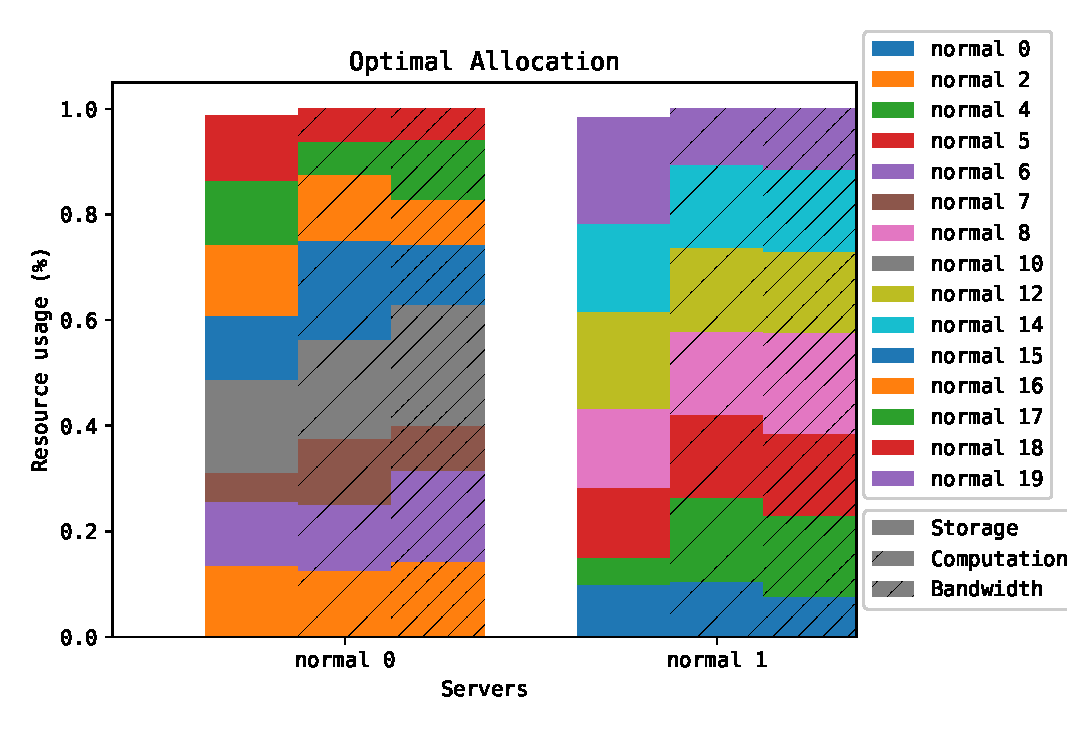
\includegraphics[width=\linewidth]{../testing/figures/allocation/eps/allocation_optimal_allocation.eps}
    \caption{Example Allocation with the optimal solution}
    \label{fig:optimal_allocation}
\end{figure}

\subsection{Greedy Mechanism}\label{subsec:greedy-mechanism}
TODO \\
Greedy mechanism is a three stage algorithm where the jobs are ranked used a value density function.
Then each jobs from the sorted job ranks are assigned to a server using a server selection function and then the
resource are allocated to the job.

\begin{figure}
    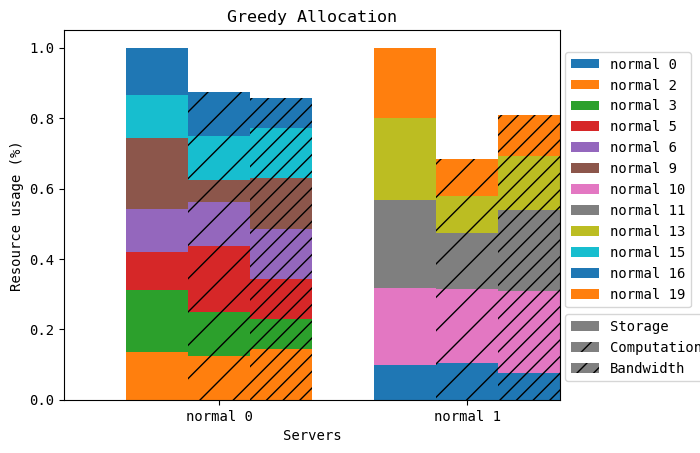
\includegraphics[width=\linewidth]{../testing/figures/allocation/png/allocation_greedy_allocation.png}
    \caption{Greedy allocation (using the same model as~\ref{fig:optimal_allocation})}
    \label{fig:greedy_allocation}
\end{figure}

\subsubsection{Greedy algorithm}
The greedy algorithm code in python
\begin{lstlisting}[language=Python]
ranked_jobs = sort(jobs, key=lambda j: value_density(j))
for job in ranked_jobs:
    allocated_server = server_selection(job, servers)

    if allocated_server:
        loading_speed, compute_speed, sending_speed = resource_allocation(job, allocated_server)
        allocate(job, allocated_server, loading_speed, compute_speed, sending_speed)
\end{lstlisting}

Example Value density function
\begin{align}
    s_j + w_j + r_j
\end{align}

Example Server selection function (where $S^{'}_i$ is the available storage for the server $i$ and $W'^{'}_i$ and $R^{'}_i$
being the avaiable computation and bandwidth respectively).
\begin{align}
    argmax_{\forall i \in I} S^{'}_i + W^{'}_i + R^{'}_i
\end{align}

Example Resource allocation function (where speeds is the set of all possible speeds that job could run at on a server)
\begin{align}
    argmin_{(s, w, r) \in speeds} s + w + r
\end{align}

\subsubsection{Lower bound of greedy mechanism}
Due to the flexible nature of jobs then when allocating jobs, to be done optimally would involved being able to know
the future allocations and then plan this jobs based on that.
However this is not possible to do there the algorithm can only guarantee that a single job can be allocated when the
jobs are ranked purely by the utility of the job.

\subsection{Decentralised Iterative Auction}\label{subsec:decentralised-iterative-auction}
The VCG auction is a well known auction that is known to be economically efficient, budget balanced and incentive compatible
by finding the price of a job by calculating the social welfare if the job didnt exist compared to when it does exist.
Job are then evaluated on how good it is for the rest of the other jobs to exist and just requires a integer programming
program which works for our problem. \\
our iterative auction uses the same idea of calculating the price based on the how its allocation affects the rest of the
jobs.
This is done through calculating through calculating the total revenue that a server will receive if the new job is
running for 0 and has the option of allocating all of the current job at their current price.
The price of the new job is equal to the difference of the old allocation revenue and the new allocation revenue
(being the price that the new job will have to offer so that the server will have as much profit) plus a small value to
make the server more revenue. \\
Because of this formulation, the server will solve a slightly different linear programming problem from the optimal
algorithm.

\begin{align}
    \max & \sum^J_j P_j (\sum^I_i x_{i,j})\label{eq:dia_objective}\\
    \mbox{s.t.} \\
    & \sum_j^J S_j x_{i,j} + S_k \leq S_i, &~ \forall i \in I,\label{eq:dia_server_storage_constraint}\\
    & \sum_j^J w_j x_{i,j} + w_k\leq W_i, &~ \forall i \in I,\label{eq:dia_server_computation_constraint}\\
    & \sum_j^J (r_j + s_j) x_{i,j} + (r_k + s_k) \leq R_i, &~ \forall i \in I,\label{eq:dia_server_communication_constraint}\\
    & \frac{s_j}{s_{i,j}} + \frac{w_j}{w_{i,j}} + \frac{r_j}{r_{i,j}} \leq \frac{D_j}{x_{i,j}}, &~ \forall{i \in I, j \in J \cup \{k\}},\label{eq:dia_job_deadline}\\
    & s_{i,j}>0, &~ \forall{i \in I, j \in J \cup \{k\}}\label{eq:dia_loading_speeds}\\
    & w_{i,j}>0, &~ \forall{i \in I, j \in J \cup \{k\}}\label{eq:dia_compute_speeds}\\
    & r_{i,j}>0, &~ \forall{i \in I, j \in J \cup \{k\}}\label{eq:dia_sending_speeds}\\
    & \sum_{i=1}^{I} x_{i,j}\leq 1, &~ \forall j \in J,\label{eq:dia_server_job_allocation}\\
    & x_{i,j} \in \{0,1\}, &~ \forall{i \in I, j \in J}\label{eq:dia_job_allocation}
\end{align}

The job price is then determined by calculating the total revenue when the job is not included and when the job is included
\begin{align}
    job\_price = revenue_{J, I} - revenue{J, I}^{k}
\end{align}

\subsubsection{Decentralised Iterative auction properties}
TODO
In auction theory then four properties are considered: Incentive Compatible, Budget balanced, truthfulness and individual
rationality.
Our auction has the properties of budget balanced (as it is a decentralised algorithm so there is no centralised,
auctioneer who receives a cut).
It also has individual rationality, TODO
However, it doesnt have incentive compatibility or truthfulness as TODO (maybe it is strategyproof )

\subsubsection{Decentralised Iterative auction code}
This is a centralised version of the code that would be decentralised
\begin{lstlisting}[language=Python]
unallocated_jobs = jobs
while len(unallocated_jobs) > 0:
    job = random.choice(unallocated_jobs)

    job_price, allocation = min(evaluate_job_price(job, server) for server in servers)

    if job_price <= job.value:
        allocate_job(job, allocation, job_price, unallocated_jobs)
    else:
        unallocated_jobs.remove(job)
\end{lstlisting}

\subsection{Critical Value Auction}\label{subsec:critical-value-auction}
TODO
Single property domain auctions~\cite{nisan2007algorithmic} allow for strategyproof (weakly-dominant incentive compatible) auction that uses
an allocation algorithm like~\ref{subsec:greedy-mechanism} that the job value is reduced till the job wouldn't be allocated.

\subsubsection{Critical Value algorithm}
The critical value algorithm that uses a custom binary search to find the point that the job is no longer allocated
\begin{lstlisting}[language=Python]
ranked_jobs = sort(jobs, key=lambda j: value_density(j))
greedy_algorithm(ranked_jobs, servers)

for job in [job for job in ranked_jobs if job.allocated]:
    lower_bound = ranked_jobs.index(job)
    upper_bound = len(ranked_jobs) - 1
    jobs = ranked_jobs.copy()

    while lower_bound < upper_bound:
        pos = floor((lower_bound + upper_bound) / 2)
        jobs.remove(job)
        jobs.insert(pos, job)

        greedy_algorithm(jobs, servers)
        if job.allocated:
            lower_bound = pos + 1
        else:
            upper_bound = pos - 1

    if lower_bound == len(ranked_jobs) - 1:
        return 0
    else:
        ranked_jobs[lower_bound].value
\end{lstlisting}

\section{Empirical Evaluation}\label{sec:empirical-evaluation}
To test the algorithms above, a mixture of synthetic models and real world data to generate our jobs and servers.
The synthetic model were generated through selecting a mean and standard deviation for each attribute for which random
jobs or servers can be generated through using the gaussian distribution.
The real world data is from two data set of Google and Alibaba from 2011 and 2018 respectively that contain the
request CPU cores, memory, local disk space, priority and the total execution time of the program.
Through this we estimate the total requirement over the program length and a deadline based on the priority and
total execution time.

\subsection{Greedy mechanism testing}\label{subsec:greedy-mechanism-testing}
For the greedy algorithm, we have also implemented the optimal solution using linear integer program solver and a
relaxed variation such that a single 'super' server is considered which has the resource size of the all other servers
combined.
\begin{figure*}
    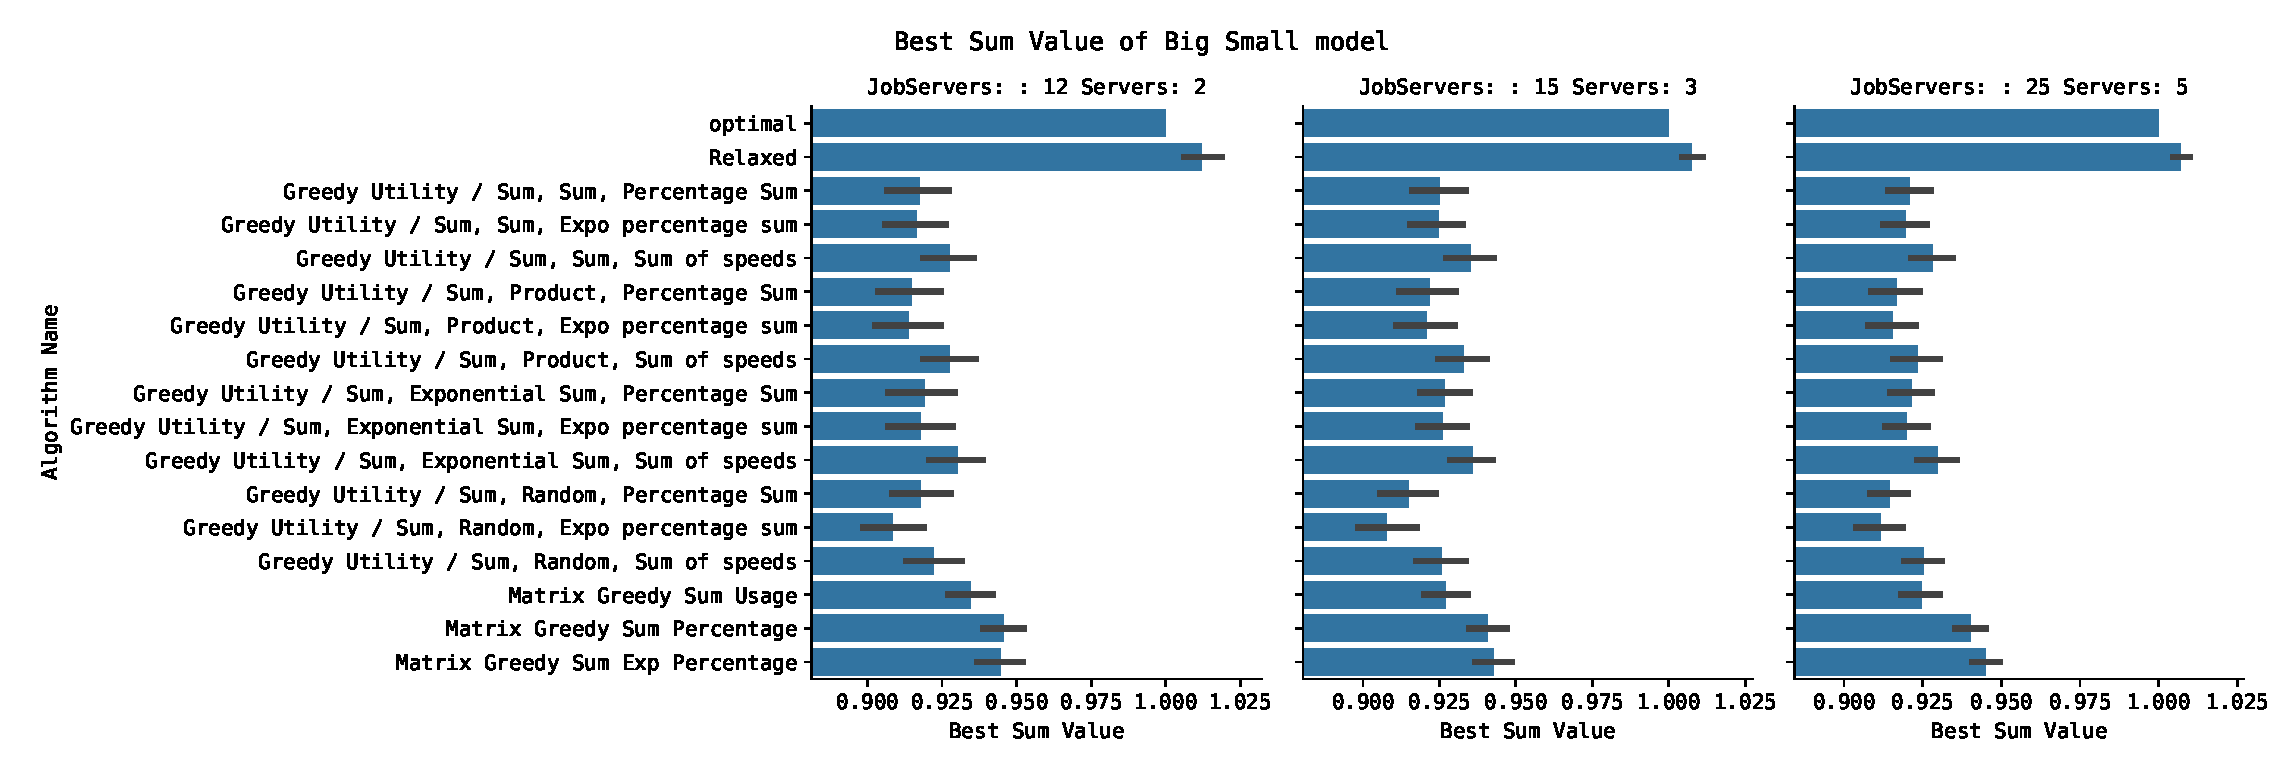
\includegraphics[width=\linewidth]{../testing/figures/greedy/eps//optimal_greedy_test_big_small_a_best_sum_value.eps}
    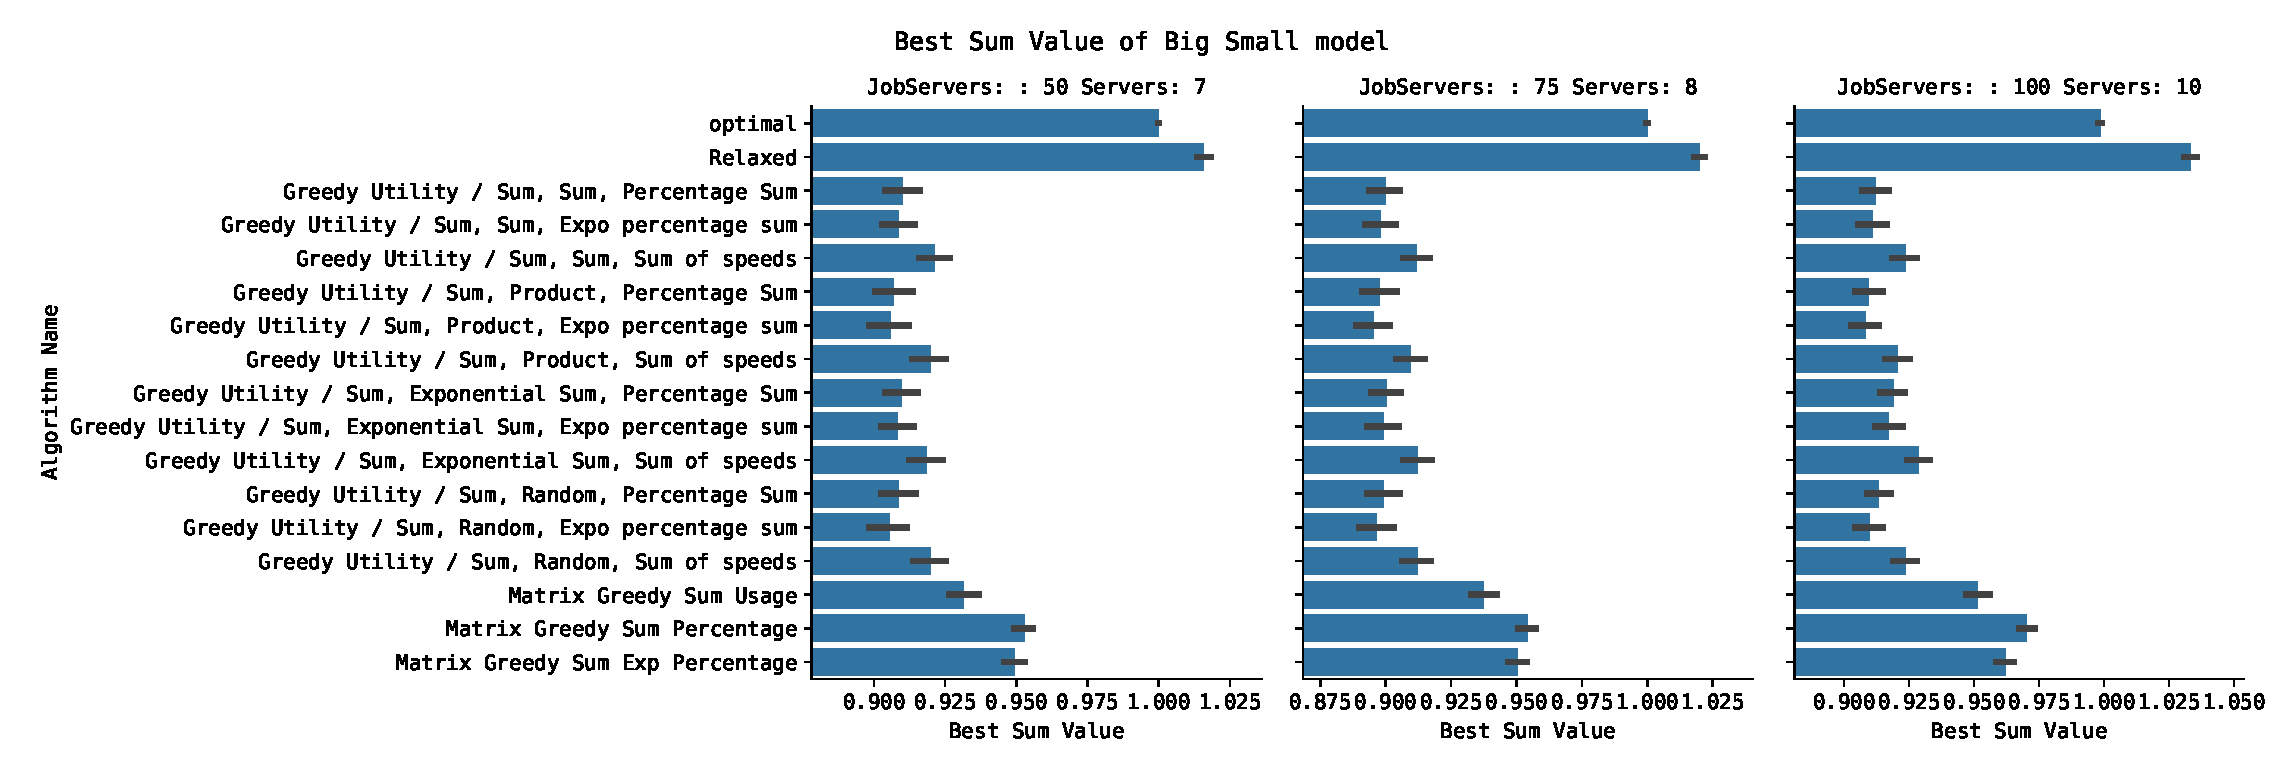
\includegraphics[width=\linewidth]{../testing/figures/greedy/eps//optimal_greedy_test_big_small_b_best_sum_value.eps}
    \caption{Greedy algorithms with big small model measuring the sum of values}
    \label{fig:big_small_sum_values}
\end{figure*}
We have found that the greedy performed within 90\% of the optimal solution for most models, it struggled the most with
settings that had high competition and so needed to be aware of other jobs requirements.
This make sense as our algorithm doesnt think about the other job requirements when allocated its current resources.

\subsection{Auction mechanisms testing}\label{subsec:auctiom-mechanisms-testing}
To test our two auction mechanisms, we have compared the results to VCG auction and a fixed VCG auction where the job speeds
are fixed before allocation.
\begin{figure}
    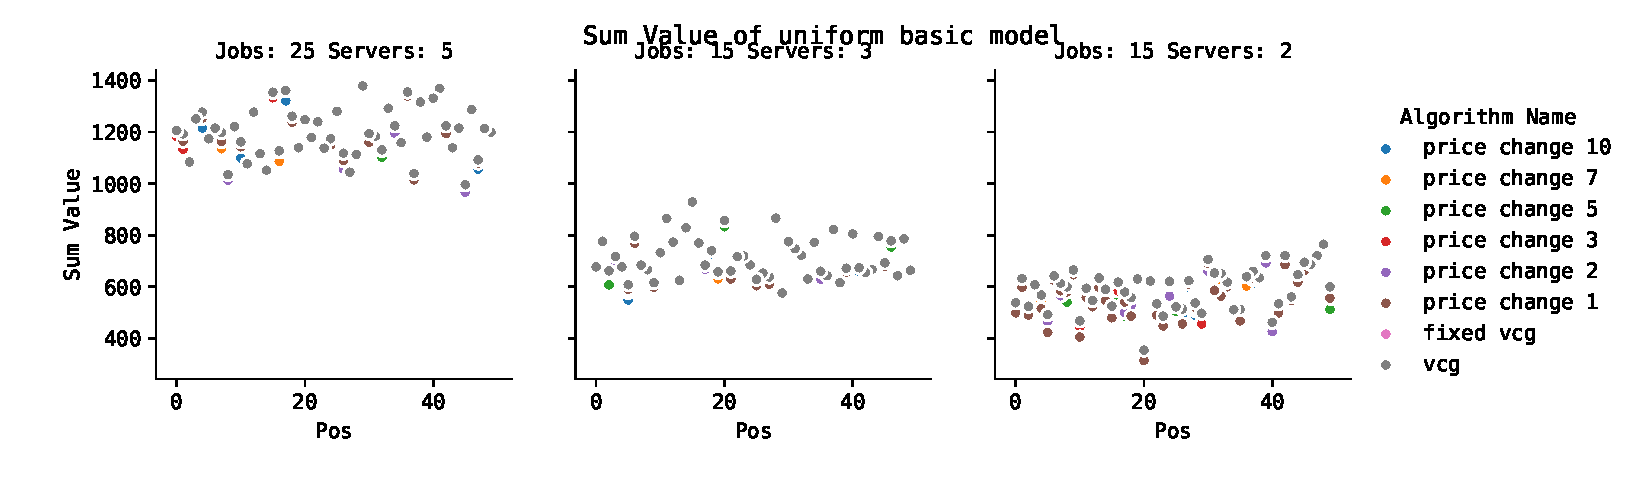
\includegraphics[width=\linewidth]{../testing/figures/price_change/eps/uniform_price_change_auction_results_basic_sum_value.eps}
    \caption{The sum value of the jobs using different algorithms}
\end{figure}

An important factor of the decentralised iterative auction is the number of rounds required till the algorithm converges
to the optimal pricing.
There are two heuristic can be used to decrease the number of round required: the price change variable and to set an
initial price for all jobs when it is first allocated.
The effect of these heuristic have a large impact on both the number of rounds and the social welfare of the allocation.
\begin{figure}
    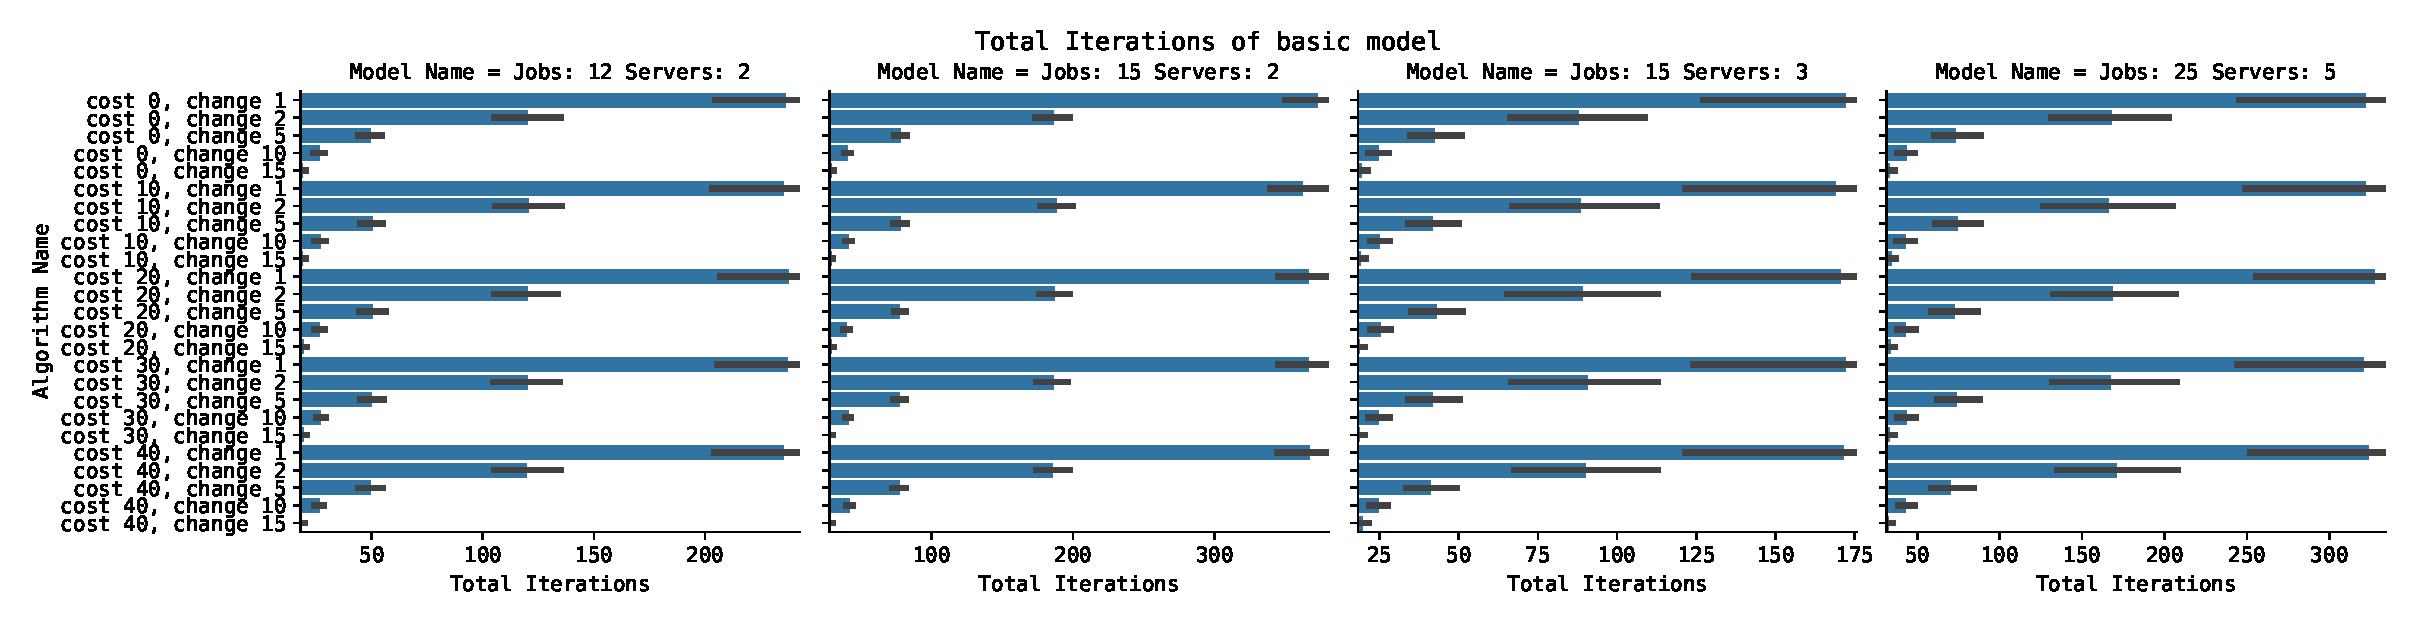
\includegraphics[width=\linewidth]{../testing/figures/iterative_round/eps/iterative_round_results_basic_total_iterations.eps}
    \caption{The number of iterative when using difference heuristics}
\end{figure}
\begin{figure}
    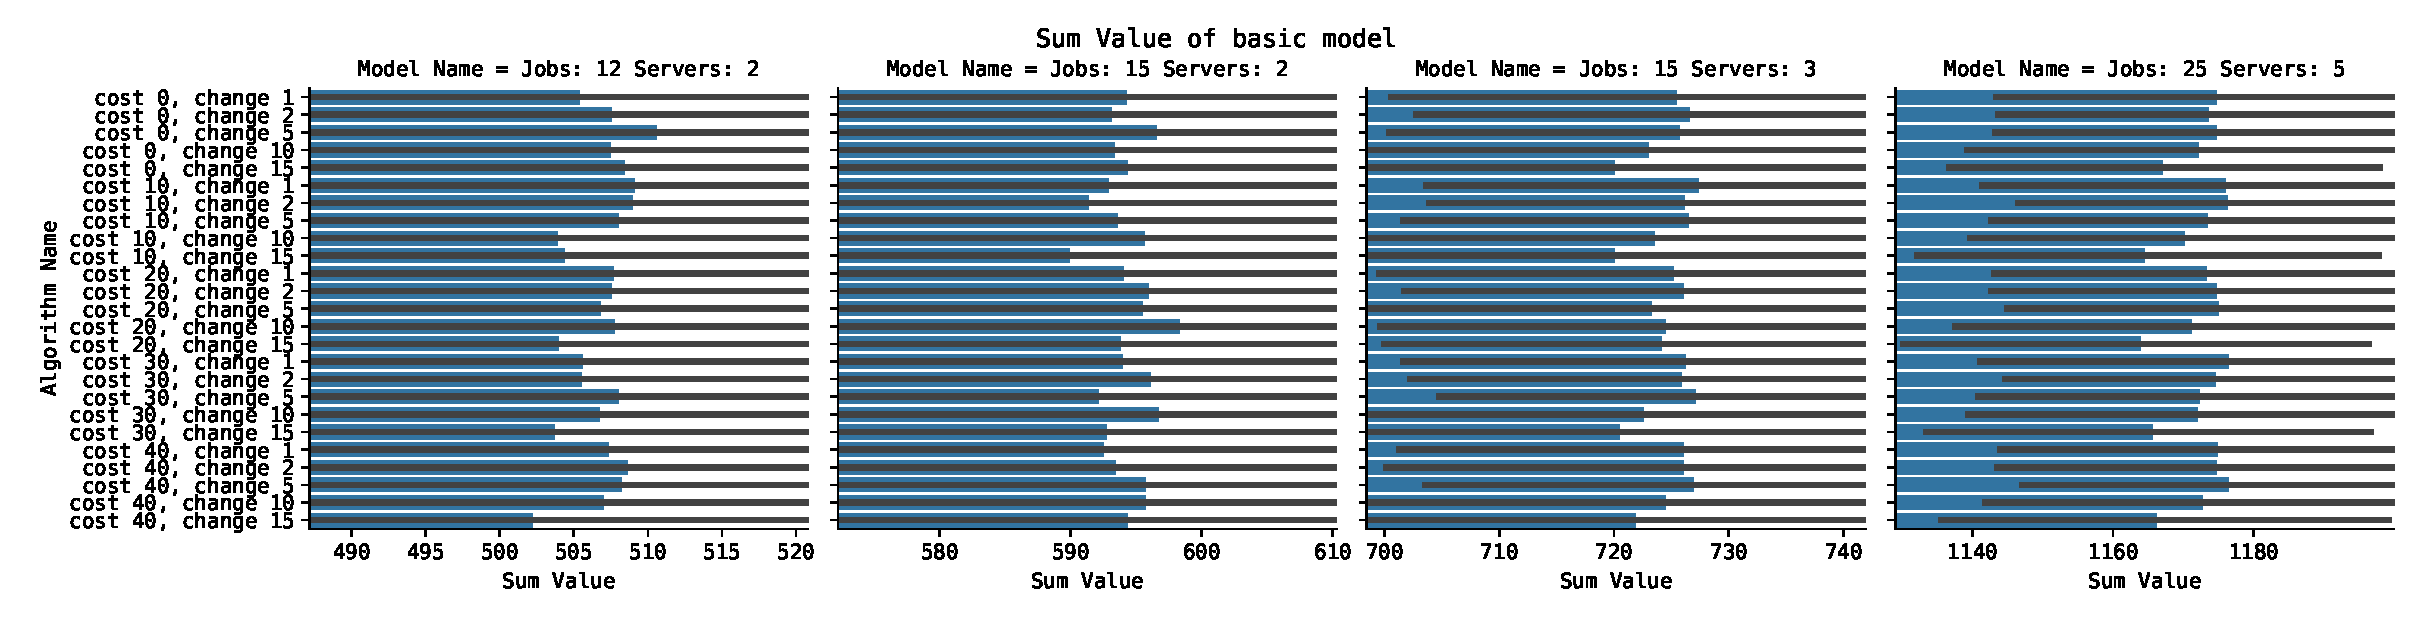
\includegraphics[width=\linewidth]{../testing/figures/iterative_round/eps/iterative_round_results_basic_sum_value.eps}
    \caption{The social welfare when using difference heuristics}
\end{figure}

To investigate if users could report worse job information and get a lower price than if they truthfully reported it.
To do this, we run the decentralised iterative auction with truthful reporting then replaced a job with a mutated version
of a job with a modified attribute.
We compared the price that job paid in comparison to the price when the job is not modified.
\begin{figure}
    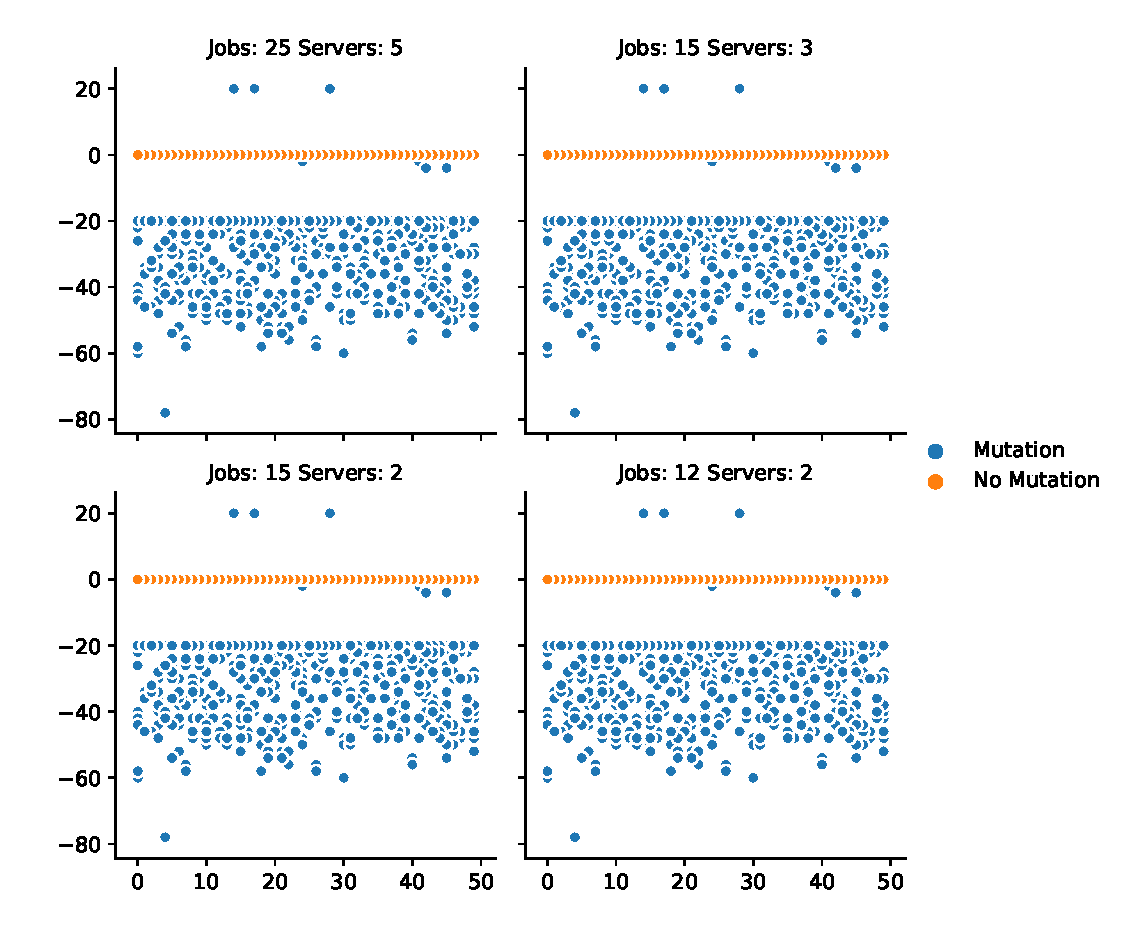
\includegraphics[width=\linewidth]{../testing/figures/auction_mutation/eps/mutate_iterative_auction_basic_mutate_difference.eps}
    \caption{Measuring the difference in price when the job is incorrectly reported}
\end{figure}
We have found that very few job would paid less when modified however we found that this can happen due to allocation
process has an element of randomness when multiple server offer the same price.
This can cause the allocation to fall into a local maximum which means that some job are allocated that otherwise wouldn't
be allocated in the global maximum of job prices.
TODO prove that this is true through running a model multiple times to see if a job is sometimes allocated and
sometimes not.

\section{Conclusions and Future Work}\label{sec:conclusions-and-future-work}
TODO

%%%%%%%%%%%%%%%%%%%%%%%%%%%%%%%%%%%%%%%%%%%%%%%%%%%%%%%%%%%%%%%%%%%%%%%%%%%%%%%%%%%%%%%%%%%%%%%%%%%%%%%%%
%% bibliography: see CFP for number of permitted pages

\bibliographystyle{ACM-Reference-Format}  % do not change this line!
\bibliography{bibliography}  % put name of your .bib file here

\end{document}
